% \begin{figure}[h]
%     \centering
%     \begin{tikzpicture}[scale=0.5]
%         \draw [blue,line width=2pt] (0,0) circle [radius=7];
%         \draw [blue,line width=1pt] (-9,0) -- (9,0);
%         \draw [blue,line width=1pt] (0,-9) -- (0,9);
%         % \draw [red, line width=1pt] (0,0)
%         % \line (1,0){10}
%     \end{tikzpicture}
%     \caption{Alternate representation of Pythagorean theorem.}
%     \label{fig:fig2}
% \end{figure}


\begin{figure}[h]
    \centering
    
    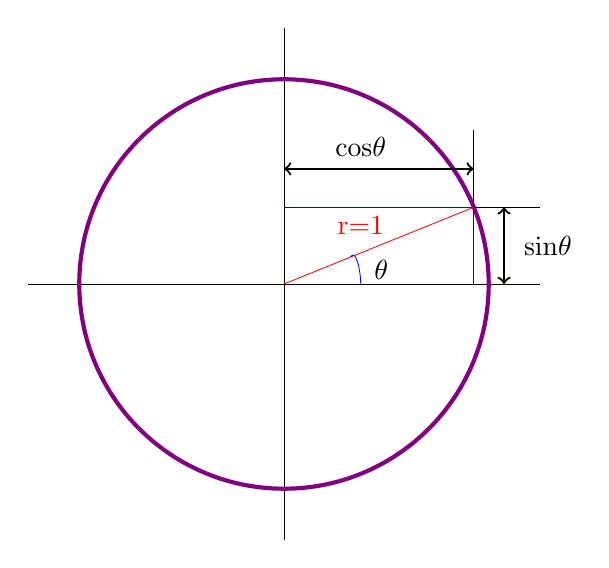
\begin{tikzpicture}[scale=0.65]

        \draw [line width=.3pt] (-5,0) -- (5,0); %x axis
        \draw [line width=.3pt] (0,-5) -- (0,5); % y axis
        
       
        \draw [violet,line width=1.5pt,circle] (0,0) circle [radius=4];
        
        \draw [blue,line width=.3pt] (0,1.5) -- (3.7081,1.5); %x axis er parallel
        \draw [black,line width=.3pt] (3.7081,1.5) -- (5,1.5); %x axis er parallel
        
        \draw [blue,line width=.3pt] (3.7081,0) -- (3.7081,1.5); %y axis er parallel
        \draw [black,line width=.3pt] (3.7081,1.5) -- (3.7081,3); %y axis er parallel
        
        \draw [red,line width=.3pt] (0,0) -- (3.7081,1.5); % r=1 line
        \node [red,below] at (1.5,1.5) {r=1};
        
        %  sin label
        
        %\draw [line width=.5pt] (4.3,0) -- (4.3,1.5);
        \draw [<-=latex,->=latex, thick] (4.3,0) -- (4.3,1.5);
        \draw [<-=latex,->=latex,thick] (4.3,1.5) -- (4.3,0);
        \node [right] at (4.5,0.75) {sin$\theta$};
        
        % cos label
        
        %\draw [line width=.5pt] (0,2.25) -- (3.7081,2.25);
        \draw [<-=latex,->=latex,thick] (0,2.25) -- (3.7081,2.25);
        \draw [<-=latex,->=latex,thick] (3.7081,2.25) -- (0,2.25);
        \node [above] at (1.5,2.3) {cos$\theta$};
        
        % theta label
        
        \draw [blue,line width=.3pt] (1.5,0) to [out=90,in=60] (1.3,.5258757854);
        \node [above] at (1.9,-0.1) {$\theta$};
        

    
    \end{tikzpicture}
    
    \caption{Alternate representation of Pythagorean theorem.}
    \label{fig:fig2}
\end{figure}